% Light Up frames — English version, \input from slides/main-en.tex.

\begin{frame}{Problem 2: Light Up (Akari)}
\begin{columns}[c,onlytextwidth]
\column{.42\textwidth}\centering
\begin{tikzpicture}[scale=.62]
  \foreach \r in {0,...,6}
    \foreach \c in {0,...,6}
      \fill[yellow!30] (\c-.5,-\r-.5) rectangle (\c+.5,-\r+.5);
  \foreach \r/\c/\v in {2/2/2,3/2/0,3/5/2,3/6/0,4/2/0,5/1/0,6/3/0,6/6/1}{
    \fill[ink!90] (\c-.5,-\r-.5) rectangle (\c+.5,-\r+.5);
    \node[white,font=\footnotesize\bfseries] at (\c,-\r) {\v};}
  \foreach \r/\c in {0/1,1/2,2/3,3/4,4/5,5/6,6/0}{
    \fill[orange!85] (\c,-\r) circle (.30);
    \fill[white] (\c,-\r) circle (.11);}
  \draw[ink!45] (-.5,.5) grid (6.5,-6.5);
\end{tikzpicture}
\column{.55\textwidth}
\begin{itemize}
\item Place bulbs on \textbf{white cells}; each bulb shines in 4 directions
until a wall or the edge.
\item Every white cell must be illuminated.
\item No two bulbs may see each other.
\item A wall numbered $k$ has exactly $k$ adjacent bulbs.
\end{itemize}
\vspace{3mm}
\small Real sample board: \texttt{akari-7-easy-70097} from the generator;\par
the picture shows its 7-bulb solution.\par
\src{Rules: puzzle-light-up.com. Board: generator/generate.py, seed 70097.}
\end{columns}
\end{frame}

\begin{frame}{Problem formulation}
\small
\begin{tabular}{@{}p{.23\textwidth}p{.70\textwidth}@{}}
\toprule
Input & Board: \texttt{None} (white), $-1$ (wall), $0..4$ (numbered wall) \\
State & Bulb set encoded as a \textbf{$W$-bit bitmask} ($W$ = white cells) \\
Initial state & Empty set (mask 0) \\
Action & Place a bulb on an eligible white cell \\
Transition & Set the bit; reject rule-breaking or unreachable successors \\
Goal & All white cells lit, all clues exact, no conflicts \\
Cost & One per placed bulb (A*'s objective) \\
\bottomrule
\end{tabular}\par
\vspace{5mm}
\normalsize Both solvers branch on the \textbf{first unlit cell (row-major)}:
only legal bulbs illuminating it are considered.\par
\small One parent per state $\Rightarrow$ no complex duplicate machinery; the
comparison between solvers stays fair.
\src{Implemented model: \_View.branch\_cell in light\_up\_problem/algorithms/search.py.}
\end{frame}

\begin{frame}{Shared sound pruning}
\centering
\begin{tikzpicture}[node distance=5mm,
 test/.style={draw=muted!45,minimum width=100mm,minimum height=7mm,font=\small},
 link/.style={-{Stealth},draw=muted}]
\node[test] (a) {Bulb on a white cell illuminating the first unlit cell};
\node[test,below=of a] (b) {No line-of-sight conflict, no overfilled clue};
\node[test,below=of b] (c) {Every clue can still reach its count};
\node[test,below=of c] (d) {No dark cell left without a possible illuminator};
\draw[link] (a)--(b);\draw[link] (b)--(c);\draw[link] (c)--(d);
\end{tikzpicture}
\vspace{3mm}\par
\small The checks only discard states that cannot reach a goal $\Rightarrow$
completeness preserved.\par
This is why ``blind'' DFS is fast on small and medium boards.
\src{Implementation: \_View.feasible() in algorithms/search.py.}
\end{frame}

\begin{frame}[fragile]{Blind search: Depth-First Search}
\begin{columns}[T,onlytextwidth]
\column{.60\textwidth}
\begin{lstlisting}
DFS(puzzle, limits):
  push mask 0 onto the stack
  while stack is not empty:
    if budget exhausted: return LIMIT
    state = stack.pop()
    if state in visited: continue
    if GOAL(state): return SOLVED(state)
    cell = FIRST_UNLIT_CELL(state)
    for c in bulbs illuminating cell:
      child = state | bit(c)
      if FEASIBLE(child): push child
  return UNSOLVABLE
\end{lstlisting}
\column{.36\textwidth}
\small LIFO stack + visited set.\par\vspace{3mm}
Fixed branching order,\par no heuristic information.\par\vspace{3mm}
Worst case $O(2^W)$ states.\par\vspace{3mm}
Returns the \textbf{first} solution --- not minimum-bulb.
\end{columns}
\src{Simplified pseudocode matches depth\_first\_search(). TIMEOUT/NODE\_LIMIT/MEMORY\_LIMIT stay distinct from UNSOLVABLE.}
\end{frame}

\begin{frame}{A*'s heuristic: three lower bounds, take the max}
\[
h(n)=\max\left\{\left\lceil \tfrac{D}{G_{\max}} \right\rceil,\;
\max_w d_w,\;\left\lceil \tfrac{\sum_w d_w}{H_{\max}} \right\rceil\right\}
\qquad f=g+h,\quad g=\#\text{bulbs}
\]
\small $D$: remaining dark cells; $G_{\max}$: most cells one legal bulb lights;\par
$d_w$: numbered wall $w$'s deficit; $H_{\max}$: most adjacencies one bulb satisfies.
\vspace{4mm}
\begin{center}
\begin{tabular}{@{}ll@{}}
\toprule
Component & Why it lower-bounds\\
\midrule
$\lceil D/G_{\max}\rceil$ & One bulb lights at most $G_{\max}$ dark cells\\
$\max_w d_w$ & A wall short by $d_w$ needs at least $d_w$ bulbs\\
$\lceil \sum_w d_w/H_{\max}\rceil$ & The total deficit needs that many bulbs\\
\bottomrule
\end{tabular}
\end{center}
\vspace{3mm}
Max of lower bounds is a lower bound $\Rightarrow$ $h$ is
\textbf{admissible} $\Rightarrow$ A* returns a \textbf{minimum-bulb} solution
when it completes.
\src{Implementation: \_View.lower\_bound() in algorithms/search.py.}
\end{frame}

\begin{frame}[fragile]{A* search}
\begin{columns}[T,onlytextwidth]
\column{.60\textwidth}
\begin{lstlisting}
ASTAR(puzzle, limits):
  push (f=h(0), g=0, mask 0) into min-heap
  best_g = {0: 0}
  while heap is not empty:
    if budget exhausted: return LIMIT
    pop state with minimum f
    if GOAL(state): return SOLVED(state)
    for c in bulbs illuminating
        FIRST_UNLIT_CELL(state):
      child = state | bit(c)
      if FEASIBLE(child) and
         g+1 < best_g.get(child, inf):
        best_g[child] = g+1
        push (g+1+h(child), g+1, child)
  return UNSOLVABLE
\end{lstlisting}
\column{.36\textwidth}
\small The min-heap keeps the \textbf{whole frontier}.\par\vspace{3mm}
The \texttt{best\_g} table fights rediscovery.\par\vspace{3mm}
Each expansion recomputes three bounds over large bitmasks.\par\vspace{3mm}
Memory can grow exponentially --- visible in the data.
\end{columns}
\src{Simplified pseudocode matches astar(). Unit costs make f monotone along paths.}
\end{frame}

\begin{frame}{Seeded inputs with a verified witness}
\begin{itemize}
\item Build a cyclic \emph{witness}: exactly one bulb per row and column.
\item Propose walls only where the witness survives; derive clue numbers from
adjacent witness bulbs.
\item Keep a wall only if the witness \emph{remains a valid solution} (checked
with the same \texttt{is\_goal\_state} used in play).
\end{itemize}
\vspace{4mm}
\begin{center}
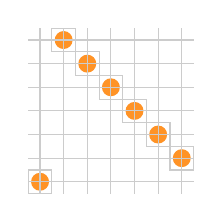
\begin{tikzpicture}[scale=.30]
  \foreach \r/\c in {0/1,1/2,2/3,3/4,4/5,5/6,6/0}{
    \draw[gray!40] (\c-.5,-\r-.5) rectangle (\c+.5,-\r+.5);
    \fill[orange!85] (\c,-\r) circle (.38);}
  \draw[gray!40] (-.5,.5) grid (6.5,-6.5);
\end{tikzpicture}
\hspace{8mm}
\begin{tabular}{@{}l@{}}
\small 4 sizes: 7, 10, 14, 25\\[1mm]
\small 3 difficulties: 16\%/10.5\%/5.5\% walls\\[1mm]
\small 12 sample sets covering all combinations\\[1mm]
\small JSON \texttt{lightup-puzzle-v1}\\[1mm]
\small \textcolor{red}{Uniqueness not checked}
\end{tabular}
\end{center}
\vspace{3mm}
\small Difficulty labels are structural (wall density), not calibrated against
solve times.
\src{Implementation: generator/generate.py. The witness is not stored in the player board.}
\end{frame}

\begin{frame}{Visual demo in pygame}
\begin{itemize}
\item \textbf{Manual play}: click to place or remove bulbs; lit cells
highlighted, conflicts outlined in red, walls show live counts.
\item \textbf{Live search}: Run / Pause / Step / Stop with expanded / generated /
frontier counters and the current bulb set (sampled events).
\item \textbf{Compare DFS and A*} on the same board: time, nodes and bulb counts
side by side.
\item \textbf{Play solution}: replay the returned placements step by step.
\end{itemize}
\vspace{4mm}
\small Solvers run in a separate spawn-safe process so the UI never stalls;\par
solver time/node/memory limits apply inside the demo too.
\src{Implementation: ui/app.py + worker.py.}
\end{frame}

\begin{frame}{Measurement protocol}
\begin{itemize}
\item 12 sample inputs: 4 sizes $\times$ 3 difficulties, 3 repeats per algorithm.
\item Limits: 30\,s, 500{,}000 nodes, 512\,MB estimated memory.
\item Same boards and limits for DFS and A*.
\end{itemize}
\vspace{4mm}
\begin{tikzpicture}[every node/.style={font=\small},node distance=24mm]
\node (map) {Seeded board};
\node[right=of map] (time) {Solver's own \texttt{perf\_counter}};
\node[right=of time] (mem) {\texttt{tracemalloc}};
\draw[-{Stealth},blue] (map)--(time);
\draw[-{Stealth},blue] (time)--(mem);
\end{tikzpicture}
\vspace{4mm}\par
\small Same machine and day as the Pipes tables (Linux, Python 3.13.14) so both
puzzles are comparable.\par
72 raw runs: \texttt{docs/benchmarks/2026-10-25-lightup.csv}.
\src{Runner: light\_up\_problem.benchmark. Evidence: docs/benchmarks/2026-10-25-lightup.md.}
\end{frame}

\begin{frame}{Results: DFS is fast and light, A* is optimal but expensive}
\small
\begin{tabular}{@{}llrrl@{}}
\toprule
Input & DFS: time / nodes & A*: time / nodes & Bulbs (DFS $\to$ A*)\\
\midrule
7 easy   & 0.026\,s / 8    & 0.273\,s / 70   & $7 = 7$\\
7 normal & 0.016\,s / 9    & 0.236\,s / 153  & $8 \to \mathbf{7}$\\
7 hard   & 0.027\,s / 7    & 6.77\,s / 3164  & $6 = 6$\\
10 easy  & 0.549\,s / 248  & 3.50\,s / 618   & $11 \to \mathbf{10}$\\
10 normal& 0.057\,s / 13   & 26.7\,s / 5464  & $12 \to \mathbf{9}$\\
10 hard  & 0.078\,s / 12   & \textcolor{red}{TIMEOUT 30\,s} (3621\,KiB) & ---\\
14 (all) & 0.35--0.42\,s / 15--17 & \textcolor{red}{TIMEOUT $\times$3} & ---\\
25 (all) & 6.7--9.7\,s / 33--35   & \textcolor{red}{TIMEOUT $\times$3} & ---\\
\bottomrule
\end{tabular}
\vspace{3mm}
\begin{itemize}
\item DFS solves \textbf{12/12} thanks to ``first unlit'' branching + pruning:
almost no backtracking (nodes $\approx$ 1.3$\times$ bulbs).
\item A* completes \textbf{5/12}, 9--250$\times$ slower, but proves optimality:
10-normal needs only 9 bulbs, not 12 (DFS overshoots 33\%).
\item Rerunning A* with a \textbf{600 s} budget: all 7 inputs still TIMEOUT
(10-hard: 151k nodes, $\sim$70 MiB) --- TIMEOUT is \emph{inconclusive}, never
unsolvable.
\end{itemize}
\src{Median of 3 runs (30 s) plus one 600 s run each, measured 25 October 2026, Linux. Data: docs/benchmarks/2026-10-25-lightup*.csv.}
\end{frame}

\begin{frame}{Limitations and next steps}
\begin{itemize}
\item Difficulty labels come from wall density, not calibrated solve times.
\item Solution uniqueness is not checked.
\item tracemalloc measures peak Python allocations, not process RSS.
\item Stronger lower bounds (matching over dark cells) could push A* further.
\end{itemize}
\vspace{5mm}
\small\textbf{References}\par\vspace{2mm}
Akari rules: \url{https://www.puzzle-light-up.com/}\par
Russell \& Norvig, \emph{Artificial Intelligence: A Modern Approach}, 4th ed.,
Chapter 3.\par
Full analysis: \texttt{docs/lightup-analysis.md}.
\end{frame}
